\documentclass[border=6pt]{standalone}
\usepackage{fontspec}
\setmainfont{TeX Gyre Termes}
\usepackage{tikz}
\usetikzlibrary{arrows.meta,positioning,shapes.geometric,shapes.multipart,fit,calc,backgrounds,shapes.misc}
\definecolor{hust}{RGB}{170,20,45}
\definecolor{navy}{RGB}{16,42,94}
\definecolor{lblue}{RGB}{225,236,250}
\definecolor{lgreen}{RGB}{226,244,232}
\definecolor{lyel}{RGB}{255,245,214}
\definecolor{lred}{RGB}{252,228,232}
\definecolor{lgray}{RGB}{242,242,242}
\tikzset{
  uc/.style={ellipse,draw=navy,fill=lblue,thick,minimum height=0.95cm,minimum width=4.4cm,align=center,font=\small,inner sep=1pt},
  arr/.style={-{Stealth[length=2.2mm]},thick},
  dep/.style={-{Stealth[length=2.2mm]},thick,dashed},
  box/.style={draw=navy,thick,rounded corners=2pt,align=center,font=\small,fill=white},
}
\newcommand{\actor}[3]{% name, pos, label
  \begin{scope}[shift={#2}]
    \draw[thick] (0,0.55) circle (0.22);
    \draw[thick] (0,0.33) -- (0,-0.25);
    \draw[thick] (-0.35,0.12) -- (0.35,0.12);
    \draw[thick] (0,-0.25) -- (-0.3,-0.7);
    \draw[thick] (0,-0.25) -- (0.3,-0.7);
    \node[font=\small\bfseries,align=center,anchor=south] (#1) at (0,0.85) {#3};
    \coordinate (#1-c) at (0,0);
    \coordinate (#1-r) at (0.38,0.12);
    \coordinate (#1-l) at (-0.38,0.12);
  \end{scope}}

\tikzset{
 pkg/.style={draw=navy,thick,fill=#1,minimum width=3.3cm,minimum height=0.9cm,font=\footnotesize\ttfamily,align=center},
 pkg/.default=lblue,
 d/.style={-{Stealth[length=2mm]},dashed,thick,navy!80},
}
\newcommand{\tab}[1]{\draw[navy,thick,fill=white] ([yshift=0pt]#1.north west) rectangle ++(1.1,0.25);}
\begin{document}
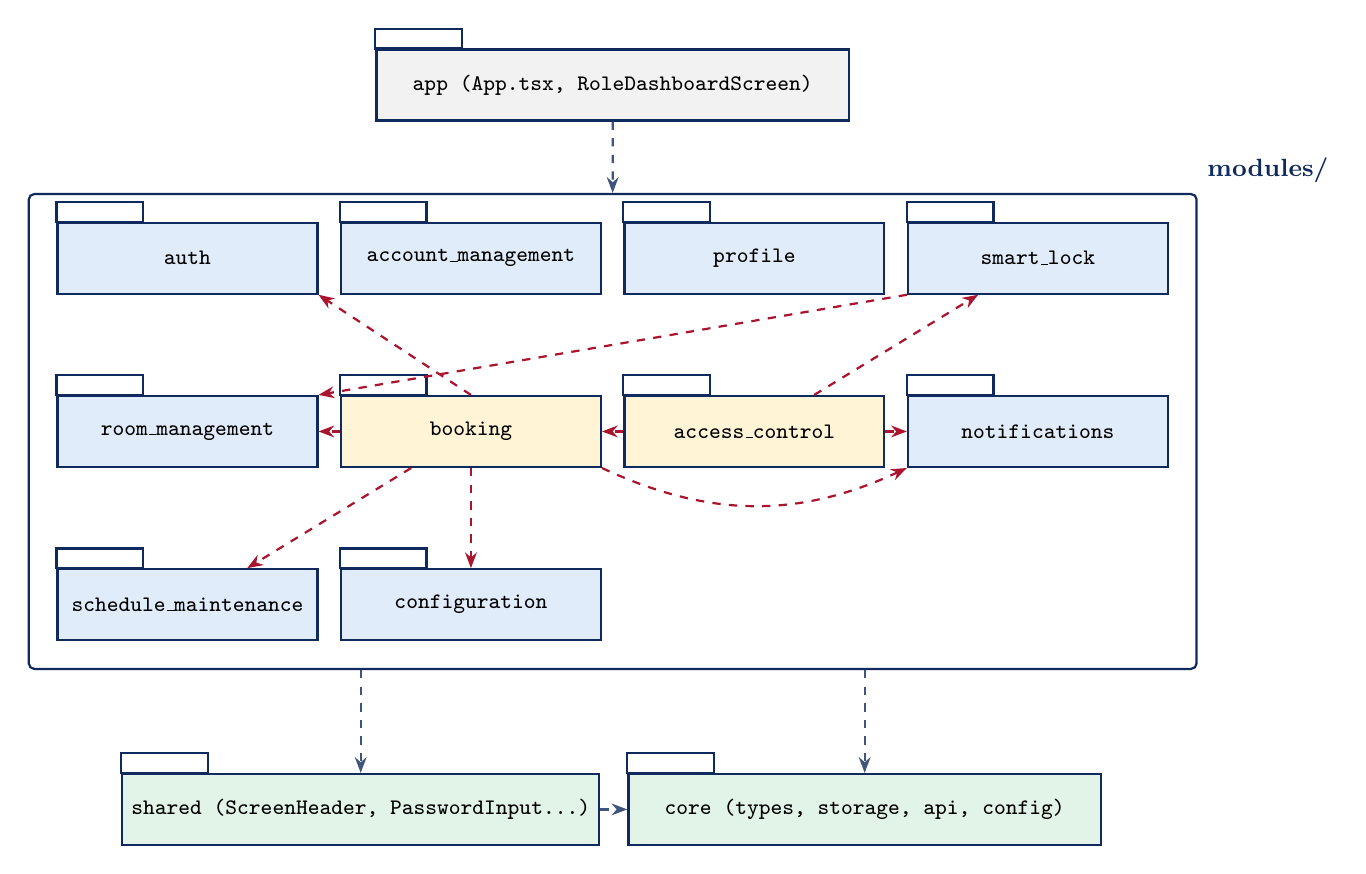
\begin{tikzpicture}
 \node[pkg=lgray,minimum width=6cm] (app) at (5.4,2.2) {app (App.tsx, RoleDashboardScreen)};
 % business modules row
 \node[pkg] (auth) at (0,0) {auth};
 \node[pkg] (acc) at (3.6,0) {account\_management};
 \node[pkg] (prof) at (7.2,0) {profile};
 \node[pkg] (lock) at (10.8,0) {smart\_lock};
 \node[pkg] (room) at (0,-2.2) {room\_management};
 \node[pkg,fill=lyel] (book) at (3.6,-2.2) {booking};
 \node[pkg,fill=lyel] (ac) at (7.2,-2.2) {access\_control};
 \node[pkg] (noti) at (10.8,-2.2) {notifications};
 \node[pkg] (maint) at (0,-4.4) {schedule\_maintenance};
 \node[pkg] (conf) at (3.6,-4.4) {configuration};
 \foreach \n in {auth,acc,prof,lock,room,book,ac,noti,maint,conf} {\tab{\n}}
 \node[draw=navy,thick,rounded corners=2pt,fit=(auth)(lock)(maint)(noti),inner sep=10pt,label={[font=\small\bfseries,text=navy]north east:modules/}] (M) {};
 \node[pkg=lgreen,minimum width=6cm] (shared) at (2.2,-7.0) {shared (ScreenHeader, PasswordInput...)};
 \node[pkg=lgreen,minimum width=6cm] (core) at (8.6,-7.0) {core (types, storage, api, config)};
 \tab{shared}\tab{core}\tab{app}
 \draw[d] (app) -- (M.north);
 \draw[d] (M.south-|shared) -- (shared);
 \draw[d] (M.south-|core) -- (core);
 \draw[d] (shared) -- (core);
 % key internal deps
 \draw[d,hust] (book) -- (room);
 \draw[d,hust] (book) -- (conf);
 \draw[d,hust] (book) -- (maint);
 \draw[d,hust] (book.north) -- (auth.south east);
 \draw[d,hust] (ac) -- (book);
 \draw[d,hust] (ac) -- (lock);
 \draw[d,hust] (ac) -- (noti);
 \draw[d,hust] (book.south east) to[bend right=25] (noti.south west);
 \draw[d,hust] (lock.south west) -- (room.north east);
\end{tikzpicture}
\end{document}
